\documentclass[journal]{IEEEtran}
\usepackage{algorithm}
\usepackage{amsmath}
\usepackage{amssymb}
\usepackage[inkscapelatex=false]{svg}
\usepackage{svg}
\usepackage{stfloats}
\usepackage{amsfonts}
\usepackage{graphicx}
\usepackage{amsmath}
\usepackage{hyperref}
\usepackage{graphicx}
\usepackage{hyperref}
\usepackage[dvips]{graphicx}
\usepackage{algorithmic}\svgsetup{
inkscapepath=i/svg-inkscape/
}
\svgpath{
{svg/}}
\begin{document}
\title{MLP based Semantic communication in Optical Fibre System- A Report}
\author{Xiaomin Cai,
      \textbf{ Supervisor} Dr Tianhua Xu
}
\markboth{Report}%
{Shell \MakeLowercase{\textit{et al.}}: Bare Demo of IEEEtran.cls for IEEE Journals}
\maketitle 
\begin{abstract}
This report explores the concept of semantic communication and its potential to enhance communication efficiency in optical fibre transmission. This work was conducted during the project secondment under the EU H2020 MSCA-RISE grant. Unlike traditional communication systems that prioritise accurate symbol transmission, semantic communication focusses on conveying the intended meaning of a message. By processing data in the semantic domain, this approach enables filtering irrelevant details and compressing data while preserving its essence. The report proposes a system design incorporating a Multilayer Perceptron (MLP) for semantic coding within an optical channel. This innovative approach demonstrates substantial improvements in communication efficiency compared to conventional methods. The training process involves a collaborative effort between the transmitter and receiver, utilising a library dataset of empirical data and corresponding pragmatic tasks. The report concludes by highlighting promising avenues for future research in semantic communication, including the use of emerging machine learning techniques, the development of comprehensive theoretical frameworks, and the creation of extensive datasets specifically tailored to semantic communication applications.
\end{abstract}

\IEEEpeerreviewmaketitle
\section{Introduction}

According to Shannon \cite{shannon_mathematical_1948}, communication could be categorised into three levels:

\textit{First level: How accurately can communication symbols be transmitted? (The technical problem) } 

\textit{Second level: How precisely do transmitted symbols convey the desired meaning? (The semantic problem) }

\textit{Third level: How effectively does the received meaning affect conduct in the desired way? (The effectiveness problem) }

\begin{figure*}[t]
    \centering
    \includesvg[width=1.9\columnwidth]{Semantic.svg}
    \caption{A simplified diagram of Semantic Communication}
    \label{Semantic}
\end{figure*}

Semantic communication is a promising new approach that aims to improve communication efficiency by transmitting the meaning of a message rather than its raw data. This is achieved by processing data in the semantic domain and extracting the intent and meaning behind the information. This approach allows for filtering out irrelevant details and compressing data while preserving its essence.
Artificial intelligence and machine learning advancements are among the most important technological supports for semantic communication development.

Optical fibre transmission has become the cornerstone of modern communication networks due to its ultra-high bandwidth, low loss, and resistance to interference. It provides a reliable channel for the rapid transmission of massive amounts of data, driving the rapid development of technologies such as the Internet and cloud computing. By introducing semantic communication technology into optical fibre transmission, the transmission efficiency and intelligence level can be further improved. Semantic communication, by understanding and processing the content of information, enables more intelligent and efficient data transmission, thus better meeting people's needs for information transmission.
The current optical communication systems focus on the reduction of bit or symbol errors, disregarding the semantic significance of digital bits. Consequently, they transmit a significant amount of unnecessary data.

A Multilayer Perceptron is a type of artificial neural network consisting of multiple layers of nodes. A layer connects each node to all nodes in the subsequent layer. MLPs are capable of learning complex patterns in data, making them a powerful tool for a wide range of applications, including classification, regression, and pattern recognition.
The basic structure of an MLP includes an input layer, one or more hidden layers, and an output layer. The input layer receives the data, the hidden layers process it and extract features, and the output layer generates the final prediction. Each node in the network performs a weighted sum of its inputs and applies an activation function to introduce non-linearity. The weights and biases in the network are adjusted during training using an optimisation algorithm like gradient descent to minimise the difference between the network's predictions and the actual values. In essence, MLPs learn to approximate complex functions by combining simple linear functions and non-linear activation functions. The number of hidden layers and the number of nodes in each layer can be adjusted to control the complexity of the model.

\section{system design and coding}

\subsection*{Channel modeling}
In my optical communication system simulation, I model several key phenomena that affect signal propagation through optical fibres. These include linear effects such as chromatic dispersion and polarisation mode dispersion, nonlinear effects like the Kerr effect and four-wave mixing, and noise introduced by optical amplifiers.

\subsubsection{Chromatic Dispersion (CD)}
Chromatic dispersion is a linear effect caused by the frequency dependence of the refractive index in optical fibres. I model this using a frequency-domain transfer function:

\begin{equation}
H_{CD}(\omega, z) = \exp(j\phi(\omega, z))
\end{equation}

where the phase is given by:

\begin{equation}
\phi(\omega, z) = -\frac{1}{2}\beta_2\omega^2z - \frac{1}{6}\beta_3\omega^3z
\end{equation}

Here, $\beta_2$ is the group velocity dispersion parameter (typically around -20 ps²/km for standard single-mode fibres at 1550 nm), and $\beta_3$ is the third-order dispersion parameter (approximately 0.1 ps³/km).

\subsubsection{Polarisation Mode Dispersion (PMD)}
PMD is a statistical effect arising from fibre birefringence. I utilise a simplified first-order PMD model with the transfer function:

\begin{equation}
H_{PMD}(\omega) = \exp(-j\omega\Delta\tau/2)
\end{equation}

where the differential group delay $\Delta\tau$ is modelled as:

\begin{equation}
\Delta\tau = D_{PMD}\sqrt{z}
\end{equation}

$D_{PMD}$ is the PMD parameter, typically around 0.1 ps/$\sqrt{\text{km}}$ for modern fibres.

\subsubsection{Kerr Effect}
The Kerr effect is a nonlinear phenomenon that includes self-phase modulation (SPM) and cross-phase modulation (XPM). I model this using a nonlinear phase shift:

\begin{equation}
\phi_{NL} = \gamma |E|^2 z
\end{equation}

where $\gamma$ is the nonlinear coefficient (typically around 1.3 W$^{-1}$km$^{-1}$ for standard single-mode fibres), $|E|^2$ is the signal power, and $z$ is the propagation distance.

\subsubsection{Four-Wave Mixing (FWM)}
FWM is a nonlinear effect resulting from the third-order susceptibility of the fibre. I employ a simplified model:

\begin{equation}
E_{FWM} = j\gamma z |E|^2 E
\end{equation}

This is a first-order approximation of the FWM effect, which in reality is more complex and depends on phase-matching conditions.

\subsubsection{Amplified Spontaneous Emission (ASE) Noise}
ASE noise is introduced by optical amplifiers. I model it as additive white Gaussian noise with power:

\begin{equation}
P_{ASE} = P_{signal} \cdot NF \cdot (G - 1)
\end{equation}

where $P_{signal}$ is the signal power, $NF$ is the noise figure (typically 3-6 dB), and $G$ is the amplifier gain.

The noise is added to the signal as complex Gaussian noise:

\begin{equation}
n(t) = n_I(t) + jn_Q(t)
\end{equation}

where $n_I(t)$ and $n_Q(t)$ are independent Gaussian processes with variance $P_{ASE}/2$.

\subsubsection{Fibre Attenuation}
Signal attenuation in the fibre is modelled using the exponential decay:

\begin{equation}
P(z) = P(0) \exp(-\alpha z)
\end{equation}

where $\alpha$ is the attenuation coefficient (typically around 0.2 dB/km at 1550 nm).

\subsubsection{Simulation Method}
\documentclass[journal]{IEEEtran}
\usepackage{algorithm}
\usepackage{amsmath}
\usepackage{amssymb}
\usepackage[inkscapelatex=false]{svg}
\usepackage{svg}
\usepackage{stfloats}
\usepackage{amsfonts}
\usepackage{graphicx}
\usepackage{amsmath}
\usepackage{hyperref}
\usepackage{graphicx}
\usepackage{hyperref}
\usepackage[dvips]{graphicx}
\usepackage{algorithmic}\svgsetup{
inkscapepath=i/svg-inkscape/
}
\svgpath{
{svg/}}
\begin{document}
\title{MLP based Semantic communication in Optical Fibre System- A Report}
\author{Xiaomin Cai,
      \textbf{ Supervisor} Dr Tianhua Xu
}
\markboth{Report}%
{Shell \MakeLowercase{\textit{et al.}}: Bare Demo of IEEEtran.cls for IEEE Journals}
\maketitle 
\begin{abstract}
This report explores the concept of semantic communication and its potential to enhance communication efficiency in optical fibre transmission. This work was conducted during the project secondment under the EU H2020 MSCA-RISE grant. Unlike traditional communication systems that prioritise accurate symbol transmission, semantic communication focusses on conveying the intended meaning of a message. By processing data in the semantic domain, this approach enables filtering irrelevant details and compressing data while preserving its essence. The report proposes a system design incorporating a Multilayer Perceptron (MLP) for semantic coding within an optical channel. This innovative approach demonstrates substantial improvements in communication efficiency compared to conventional methods. The training process involves a collaborative effort between the transmitter and receiver, utilising a library dataset of empirical data and corresponding pragmatic tasks. The report concludes by highlighting promising avenues for future research in semantic communication, including the use of emerging machine learning techniques, the development of comprehensive theoretical frameworks, and the creation of extensive datasets specifically tailored to semantic communication applications.
\end{abstract}

\IEEEpeerreviewmaketitle
\section{Introduction}

According to Shannon \cite{shannon_mathematical_1948}, communication could be categorised into three levels:

\textit{First level: How accurately can communication symbols be transmitted? (The technical problem) } 

\textit{Second level: How precisely do transmitted symbols convey the desired meaning? (The semantic problem) }

\textit{Third level: How effectively does the received meaning affect conduct in the desired way? (The effectiveness problem) }

\begin{figure*}[t]
    \centering
    \includesvg[width=1.9\columnwidth]{Semantic.svg}
    \caption{A simplified diagram of Semantic Communication}
    \label{Semantic}
\end{figure*}

Semantic communication is a promising new approach that aims to improve communication efficiency by transmitting the meaning of a message rather than its raw data. This is achieved by processing data in the semantic domain and extracting the intent and meaning behind the information. This approach allows for filtering out irrelevant details and compressing data while preserving its essence.
Artificial intelligence and machine learning advancements are among the most important technological supports for semantic communication development.

Optical fibre transmission has become the cornerstone of modern communication networks due to its ultra-high bandwidth, low loss, and resistance to interference. It provides a reliable channel for the rapid transmission of massive amounts of data, driving the rapid development of technologies such as the Internet and cloud computing. By introducing semantic communication technology into optical fibre transmission, the transmission efficiency and intelligence level can be further improved. Semantic communication, by understanding and processing the content of information, enables more intelligent and efficient data transmission, thus better meeting people's needs for information transmission.
The current optical communication systems focus on the reduction of bit or symbol errors, disregarding the semantic significance of digital bits. Consequently, they transmit a significant amount of unnecessary data.

A Multilayer Perceptron is a type of artificial neural network consisting of multiple layers of nodes. A layer connects each node to all nodes in the subsequent layer. MLPs are capable of learning complex patterns in data, making them a powerful tool for a wide range of applications, including classification, regression, and pattern recognition.
The basic structure of an MLP includes an input layer, one or more hidden layers, and an output layer. The input layer receives the data, the hidden layers process it and extract features, and the output layer generates the final prediction. Each node in the network performs a weighted sum of its inputs and applies an activation function to introduce non-linearity. The weights and biases in the network are adjusted during training using an optimisation algorithm like gradient descent to minimise the difference between the network's predictions and the actual values. In essence, MLPs learn to approximate complex functions by combining simple linear functions and non-linear activation functions. The number of hidden layers and the number of nodes in each layer can be adjusted to control the complexity of the model.

\section{system design and coding}

\subsection*{Channel modeling}
In my optical communication system simulation, I model several key phenomena that affect signal propagation through optical fibres. These include linear effects such as chromatic dispersion and polarisation mode dispersion, nonlinear effects like the Kerr effect and four-wave mixing, and noise introduced by optical amplifiers.

\subsubsection{Chromatic Dispersion (CD)}
Chromatic dispersion is a linear effect caused by the frequency dependence of the refractive index in optical fibres. I model this using a frequency-domain transfer function:

\begin{equation}
H_{CD}(\omega, z) = \exp(j\phi(\omega, z))
\end{equation}

where the phase is given by:

\begin{equation}
\phi(\omega, z) = -\frac{1}{2}\beta_2\omega^2z - \frac{1}{6}\beta_3\omega^3z
\end{equation}

Here, $\beta_2$ is the group velocity dispersion parameter (typically around -20 ps²/km for standard single-mode fibres at 1550 nm), and $\beta_3$ is the third-order dispersion parameter (approximately 0.1 ps³/km).

\subsubsection{Polarisation Mode Dispersion (PMD)}
PMD is a statistical effect arising from fibre birefringence. I utilise a simplified first-order PMD model with the transfer function:

\begin{equation}
H_{PMD}(\omega) = \exp(-j\omega\Delta\tau/2)
\end{equation}

where the differential group delay $\Delta\tau$ is modelled as:

\begin{equation}
\Delta\tau = D_{PMD}\sqrt{z}
\end{equation}

$D_{PMD}$ is the PMD parameter, typically around 0.1 ps/$\sqrt{\text{km}}$ for modern fibres.

\subsubsection{Kerr Effect}
The Kerr effect is a nonlinear phenomenon that includes self-phase modulation (SPM) and cross-phase modulation (XPM). I model this using a nonlinear phase shift:

\begin{equation}
\phi_{NL} = \gamma |E|^2 z
\end{equation}

where $\gamma$ is the nonlinear coefficient (typically around 1.3 W$^{-1}$km$^{-1}$ for standard single-mode fibres), $|E|^2$ is the signal power, and $z$ is the propagation distance.

\subsubsection{Four-Wave Mixing (FWM)}
FWM is a nonlinear effect resulting from the third-order susceptibility of the fibre. I employ a simplified model:

\begin{equation}
E_{FWM} = j\gamma z |E|^2 E
\end{equation}

This is a first-order approximation of the FWM effect, which in reality is more complex and depends on phase-matching conditions.

\subsubsection{Amplified Spontaneous Emission (ASE) Noise}
ASE noise is introduced by optical amplifiers. I model it as additive white Gaussian noise with power:

\begin{equation}
P_{ASE} = P_{signal} \cdot NF \cdot (G - 1)
\end{equation}

where $P_{signal}$ is the signal power, $NF$ is the noise figure (typically 3-6 dB), and $G$ is the amplifier gain.

The noise is added to the signal as complex Gaussian noise:

\begin{equation}
n(t) = n_I(t) + jn_Q(t)
\end{equation}

where $n_I(t)$ and $n_Q(t)$ are independent Gaussian processes with variance $P_{ASE}/2$.

\subsubsection{Fibre Attenuation}
Signal attenuation in the fibre is modelled using the exponential decay:

\begin{equation}
P(z) = P(0) \exp(-\alpha z)
\end{equation}

where $\alpha$ is the attenuation coefficient (typically around 0.2 dB/km at 1550 nm).

\subsubsection{Simulation Method}
In my simulation, I employ the split-step Fourier method to combine these effects. The fibre is divided into small segments (typically 0.1 km), and linear effects are applied in the frequency domain whilst nonlinear effects are applied in the time domain for each segment.

The choice of parameters in my simulation is based on typical values for standard single-mode fibres operating at 1550 nm. However, these parameters can be adjusted to model different fibre types or transmission scenarios. The simulation provides a comprehensive framework for studying the interplay between various optical effects and their impact on signal propagation in fibre-optic communication systems.
In this report, I utilised semantic communication in a optical channel with MLP, resulting in a substantial enhancement in communication efficiency. The results shows that given equivalent bandwidth, the effective data transmission capacity can be significantly higher compared to traditional fibre optics.



As shown in Algorithm 1,
there is a dataset called library dataset $\mathcal{K}$, which is a collection of empirical data $K$ and its corresponding pragmatic task $Z$ from background knowledge. The transmitter and receiver train the coder networks collectively with the empirical data $K$.
In this approach, the data converting function, the encoding function, and the decoding functions, namely $G_{K}(\cdot)$, $f(\cdot)$, $g(\cdot)$, are all realized by neural networks. Meanwhile, in this report, the pragmatic function $\phi(\cdot)$ is set as a given one. It can be regarded as the mathematical abstraction of the pragmatic task, while how to obtain it is not the focus of this algorithm. And the data set for training and testing is MNIST.

Initially, the encoder $f(\cdot)$ and the decoder $g(\cdot)$ are jointly trained, based on the library dataset $\cal K$. The joint source-channel coding (JSCC)-based semantic communication in this report can also be regarded as task-orientated semantic communication \cite{gunduz_beyond_2023,guler_semantic_2018}. Hence, the encoder $f(\cdot)$ aims to extract and transmit the data containing most semantic information and observable information, while the decoder $g(\cdot)$ aims to reconstruct the data related to the pragmatic task and the empirical data. Also mentioned in \cite{xie_task-oriented_2022-1,shi_semantic_2021}, the coders take into account both the semantic information and channel influence.







\begin{algorithm}[t]
\fontsize{10pt}{11pt}\selectfont
\caption{semantic coding training algorithm.}
\label{preliminary_traning}
\begin{algorithmic}[1]
\STATE Set epoch counter $t=1$.
\WHILE{the training stop condition is not met}
\STATE Take a batch of the samples $\mathcal{K}_t \subset \mathcal{K}$ (transmitter)
\STATE Encode and send all $X= f_{\boldsymbol{\theta}_1,t}\left(K\right)$ in $\mathcal{K}_t$ (transmitter).
\STATE Decode data $ \widehat{K} = g_{\boldsymbol{\theta}_2,t}\left(Y\right)$ (receiver).
\STATE $\widehat{Z} = \phi\left(\widehat{K}\right) $ (receiver).
\STATE Calculate the gradients $ \nabla_{\boldsymbol{\theta}_2} \mathcal{L}(T) $ and update $g_{\boldsymbol{\theta}_2}(\cdot)$ (receiver).
\STATE Calculate the gradient $ \nabla_{Y} \mathcal{L}$ (receiver).
\STATE Sends  $ \nabla_{Y} \mathcal{L} $ and $Y$ to the transmitter (receiver).
\STATE Calculate $\mathbb{E}_{\sim \mathcal{T}_t}\left[\nabla_{\boldsymbol{\theta}_1} \mathcal{L}\right]$ and update $f_{\boldsymbol{\theta}_1}\left(\cdot\right)$ (transmitter).

\STATE $ t=t+1 $.
\ENDWHILE

\end{algorithmic}
\end{algorithm}

\begin{figure}
    \centering
    \includegraphics[width=1\linewidth]{1.png}
    \caption{Training and Evaluation Accuracy Comparison}
    \label{1}
\end{figure}


\subsection*{Semantic training}

This section details the process of training and evaluating a MLP model on the MNIST dataset, with a focus on the integration of an optical channel model. The MNIST dataset consists of handwritten digit images, and the goal is to classify these images into one of ten digit classes (0-9). The process involves encoding the images, transmitting them through an optical channel, and then decoding and classifying them.

\subsubsection*{Data Preparation}

The MNIST dataset is loaded and preprocessed. Each image is normalized to have pixel values between -1 and 1. This normalization is achieved by first scaling the pixel values to the range [0, 1] and then applying the transformation:

\[
x = \frac{x - 0.5}{0.5}
\]

where \( x \) represents the pixel value.

\subsubsection*{Model Architecture}

The MLP model consists of two main components: an encoder-decoder network and a classifier network.

\paragraph{}{Encoder-Decoder Network}

The encoder-decoder network compresses the input image into a lower-dimensional representation and then reconstructs the image from this representation. The encoder reduces the dimensionality of the input image, while the decoder attempts to reconstruct the original image from the compressed representation.

Let \( x \) be the input image, and \( z \) be the compressed representation. The encoder can be represented as:

\[
z = f_{\text{enc}}(x)
\]

where \( f_{\text{enc}} \) is the encoding function. The decoder reconstructs the image as:

\[
\hat{x} = f_{\text{dec}}(z)
\]

where \( f_{\text{dec}} \) is the decoding function.

\paragraph{}{Classifier Network}

The classifier network takes the reconstructed image as input and outputs the class probabilities. The classifier can be represented as:

\[
y = f_{\text{cls}}(\hat{x})
\]

where \( f_{\text{cls}} \) is the classification function, and \( y \) is the output class probabilities.

\subsubsection*{Optical Channel Model}

The compressed representation \( z \) is transmitted through an optical channel, which introduces noise and distortions. The optical channel model includes various parameters such as signal-to-noise ratio, amplified spontaneous emission power, chromatic dispersion parameter, polarization mode dispersion parameter, Kerr nonlinearity coefficient, fiber length, channel spacing, phase noise variance, effective area, and wavelength.

The transmitted signal \( z' \) can be represented as:

\[
z' = \text{apply\_optical\_channel}(z)
\]

where \( \text{apply\_optical\_channel} \) is the function modeling the optical channel.

\subsubsection*{Loss Function}

The loss function used for training the model is a combination of cross-entropy loss and mean squared error (MSE) loss. The cross-entropy loss measures the classification error, while the MSE loss measures the reconstruction error. The total loss \( L \) is given by:

\[
L = \lambda_1 \cdot \text{CrossEntropyLoss}(y, y_{\text{true}}) + \lambda_2 \cdot \text{MSELoss}(\hat{x}, x)
\]

where \( \lambda_1 \) and \( \lambda_2 \) are weighting factors, \( y_{\text{true}} \) is the true class label, and \( \hat{x} \) is the reconstructed image.

\subsubsection*{Training Process}

The training process involves iterating over the training dataset for a specified number of epochs. In each epoch, the following steps are performed:

\begin{enumerate}
    \item \textbf{Forward Pass}: The input image \( x \) is encoded to obtain \( z \), transmitted through the optical channel to obtain \( z' \), and then decoded to obtain \( \hat{x} \). The classifier network then predicts the class probabilities \( y \) from \( \hat{x} \).
    \item \textbf{Loss Calculation}: The total loss \( L \) is calculated using the cross-entropy loss and MSE loss.
    \item \textbf{Backward Pass}: The gradients of the loss with respect to the model parameters are computed, and the model parameters are updated using an optimizer (e.g., SGD or Adam).
    \item \textbf{Accuracy Calculation}: The accuracy of the classifier is calculated by comparing the predicted class labels with the true class labels.
\end{enumerate}

\subsubsection*{Evaluation}

The model is evaluated on a separate test dataset. The evaluation metrics include the loss and accuracy on the test dataset. Additionally, the Peak Signal-to-Noise Ratio (PSNR) is calculated to measure the quality of the reconstructed images. The PSNR is given by:

\[
\text{PSNR} = 10 \cdot \log_{10} \left( \frac{\max(x)^2}{\text{MSE}(\hat{x}, x)} \right)
\]

where \( \max(x) \) is the maximum pixel value in the original image, and \( \text{MSE}(\hat{x}, x) \) is the mean squared error between the reconstructed and original images.

\subsubsection*{Results and Visualization}

The training and evaluation accuracies are plotted over the epochs to visualize the model's performance. Additionally, the number of reconstructed images and the efficiency ratio (encoded/raw) are plotted to compare the performance of the encoded and raw data transmission.

This section presents a detailed process of training and evaluating an MLP model on the MNIST dataset with an integrated optical channel model. The combination of cross-entropy and MSE losses ensures that the model not only classifies the images accurately but also reconstructs them with high fidelity. The evaluation metrics and visualizations provide insights into the model's performance and the impact of the optical channel on the transmitted data.











\subsection{Autoencoder Implementation}
Autoencoders are a type of artificial neural network used to learn efficient codings of unlabeled data. They are primarily used for dimensionality reduction and feature learning. This report delves into the specifics of implementing an autoencoder, providing a detailed explanation of the code and its functionality. Note that this is an ongoing research project, and the simulations may not be perfect, with room for code improvements.

\subsubsection{Code Explanation}
The implementation of an autoencoder typically involves defining the architecture, training the model, and evaluating its performance. Below is a simplified version of the code used to implement an autoencoder.

\paragraph{Architecture Definition}
The architecture of an autoencoder consists of an encoder and a decoder. The encoder compresses the input into a latent-space representation, while the decoder reconstructs the input from this representation.

\begin{algorithm}
\caption{Autoencoder Architecture Definition}
\begin{algorithmic}[1]
\State \textbf{import} tensorflow as tf
\State \textbf{from} tensorflow.keras \textbf{import} layers, models

\State \textbf{Define the encoder}
\State encoder = models.Sequential([
    layers.Input(shape=(input_dim,)),
    layers.Dense(128, activation='relu'),
    layers.Dense(64, activation='relu'),
    layers.Dense(latent_dim, activation='relu')
])

\State \textbf{Define the decoder}
\State decoder = models.Sequential([
    layers.Input(shape=(latent_dim,)),
    layers.Dense(64, activation='relu'),
    layers.Dense(128, activation='relu'),
    layers.Dense(input_dim, activation='sigmoid')
])

\State \textbf{Combine encoder and decoder into an autoencoder model}
\State autoencoder = models.Model(inputs=encoder.input, outputs=decoder(encoder.output))
\State autoencoder.compile(optimizer='adam', loss='mse')
\end{algorithmic}
\end{algorithm}

\paragraph{Training the Model}
The model is trained using the mean squared error (MSE) loss function and the Adam optimizer.

\begin{algorithm}
\caption{Training the Autoencoder}
\begin{algorithmic}[1]
\State \textbf{Train the autoencoder}
\State history = autoencoder.fit(x_train, x_train, epochs=50, batch_size=256, validation_split=0.2)
\end{algorithmic}
\end{algorithm}

\paragraph{Evaluating the Model}
After training, the model's performance is evaluated by comparing the original input with the reconstructed output.

\begin{algorithm}
\caption{Evaluating the Autoencoder}
\begin{algorithmic}[1]
\State \textbf{Evaluate the autoencoder}
\State reconstructed = autoencoder.predict(x_test)
\State mse = np.mean(np.power(x_test - reconstructed, 2), axis=1)
\end{algorithmic}
\end{algorithm}

\subsubsection{Results and Discussion}
The performance of the autoencoder can be visualised using various metrics. In this report, we use the magnitude distribution and the reconstruction error.

\paragraph{Magnitude Distribution}
The magnitude distribution of the latent-space representation provides insights into the encoding efficiency. Figure \ref{fig:magnitude_distribution} shows the magnitude distribution.

\begin{figure}
    \centering
    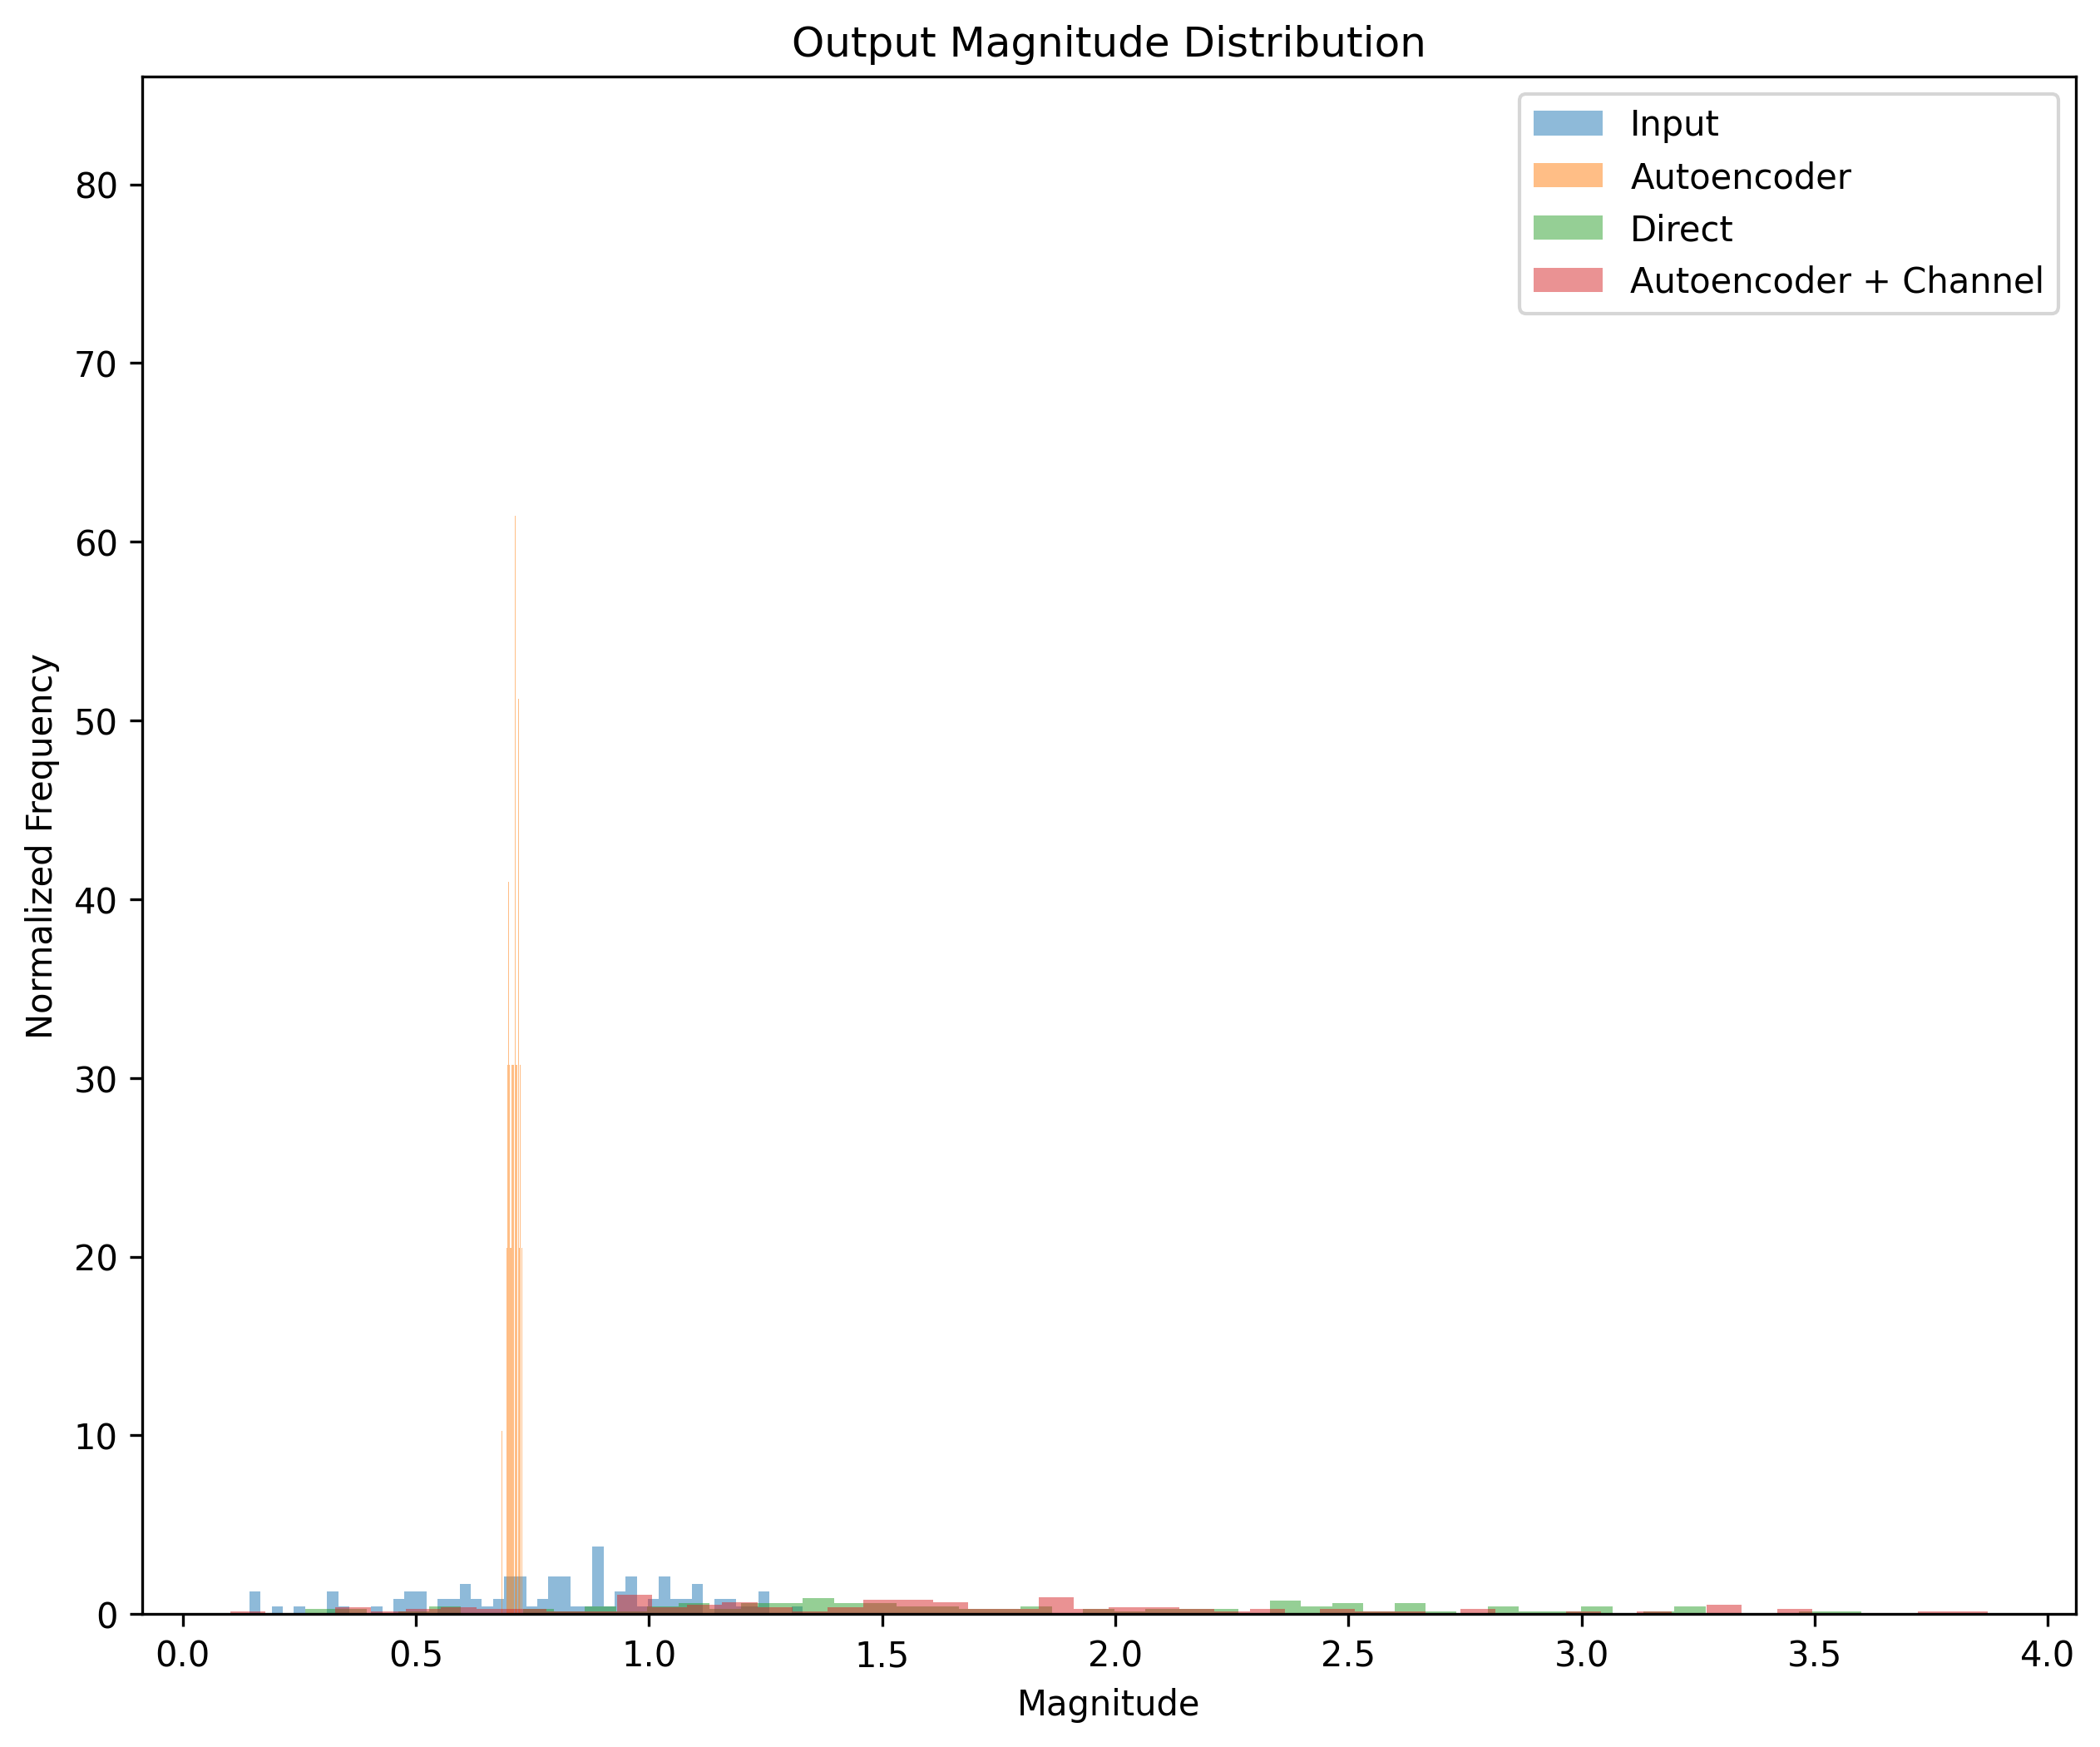
\includegraphics[width=1\linewidth]{magnitude_distribution.png}
    \caption{Magnitude Distribution of Latent-Space Representation}
    \label{fig:magnitude_distribution}
\end{figure}

\paragraph{Autoencoder Comparison}
Figure \ref{fig:autoencoder_comparison} compares the performance of the autoencoder with other models.

\begin{figure}
    \centering
    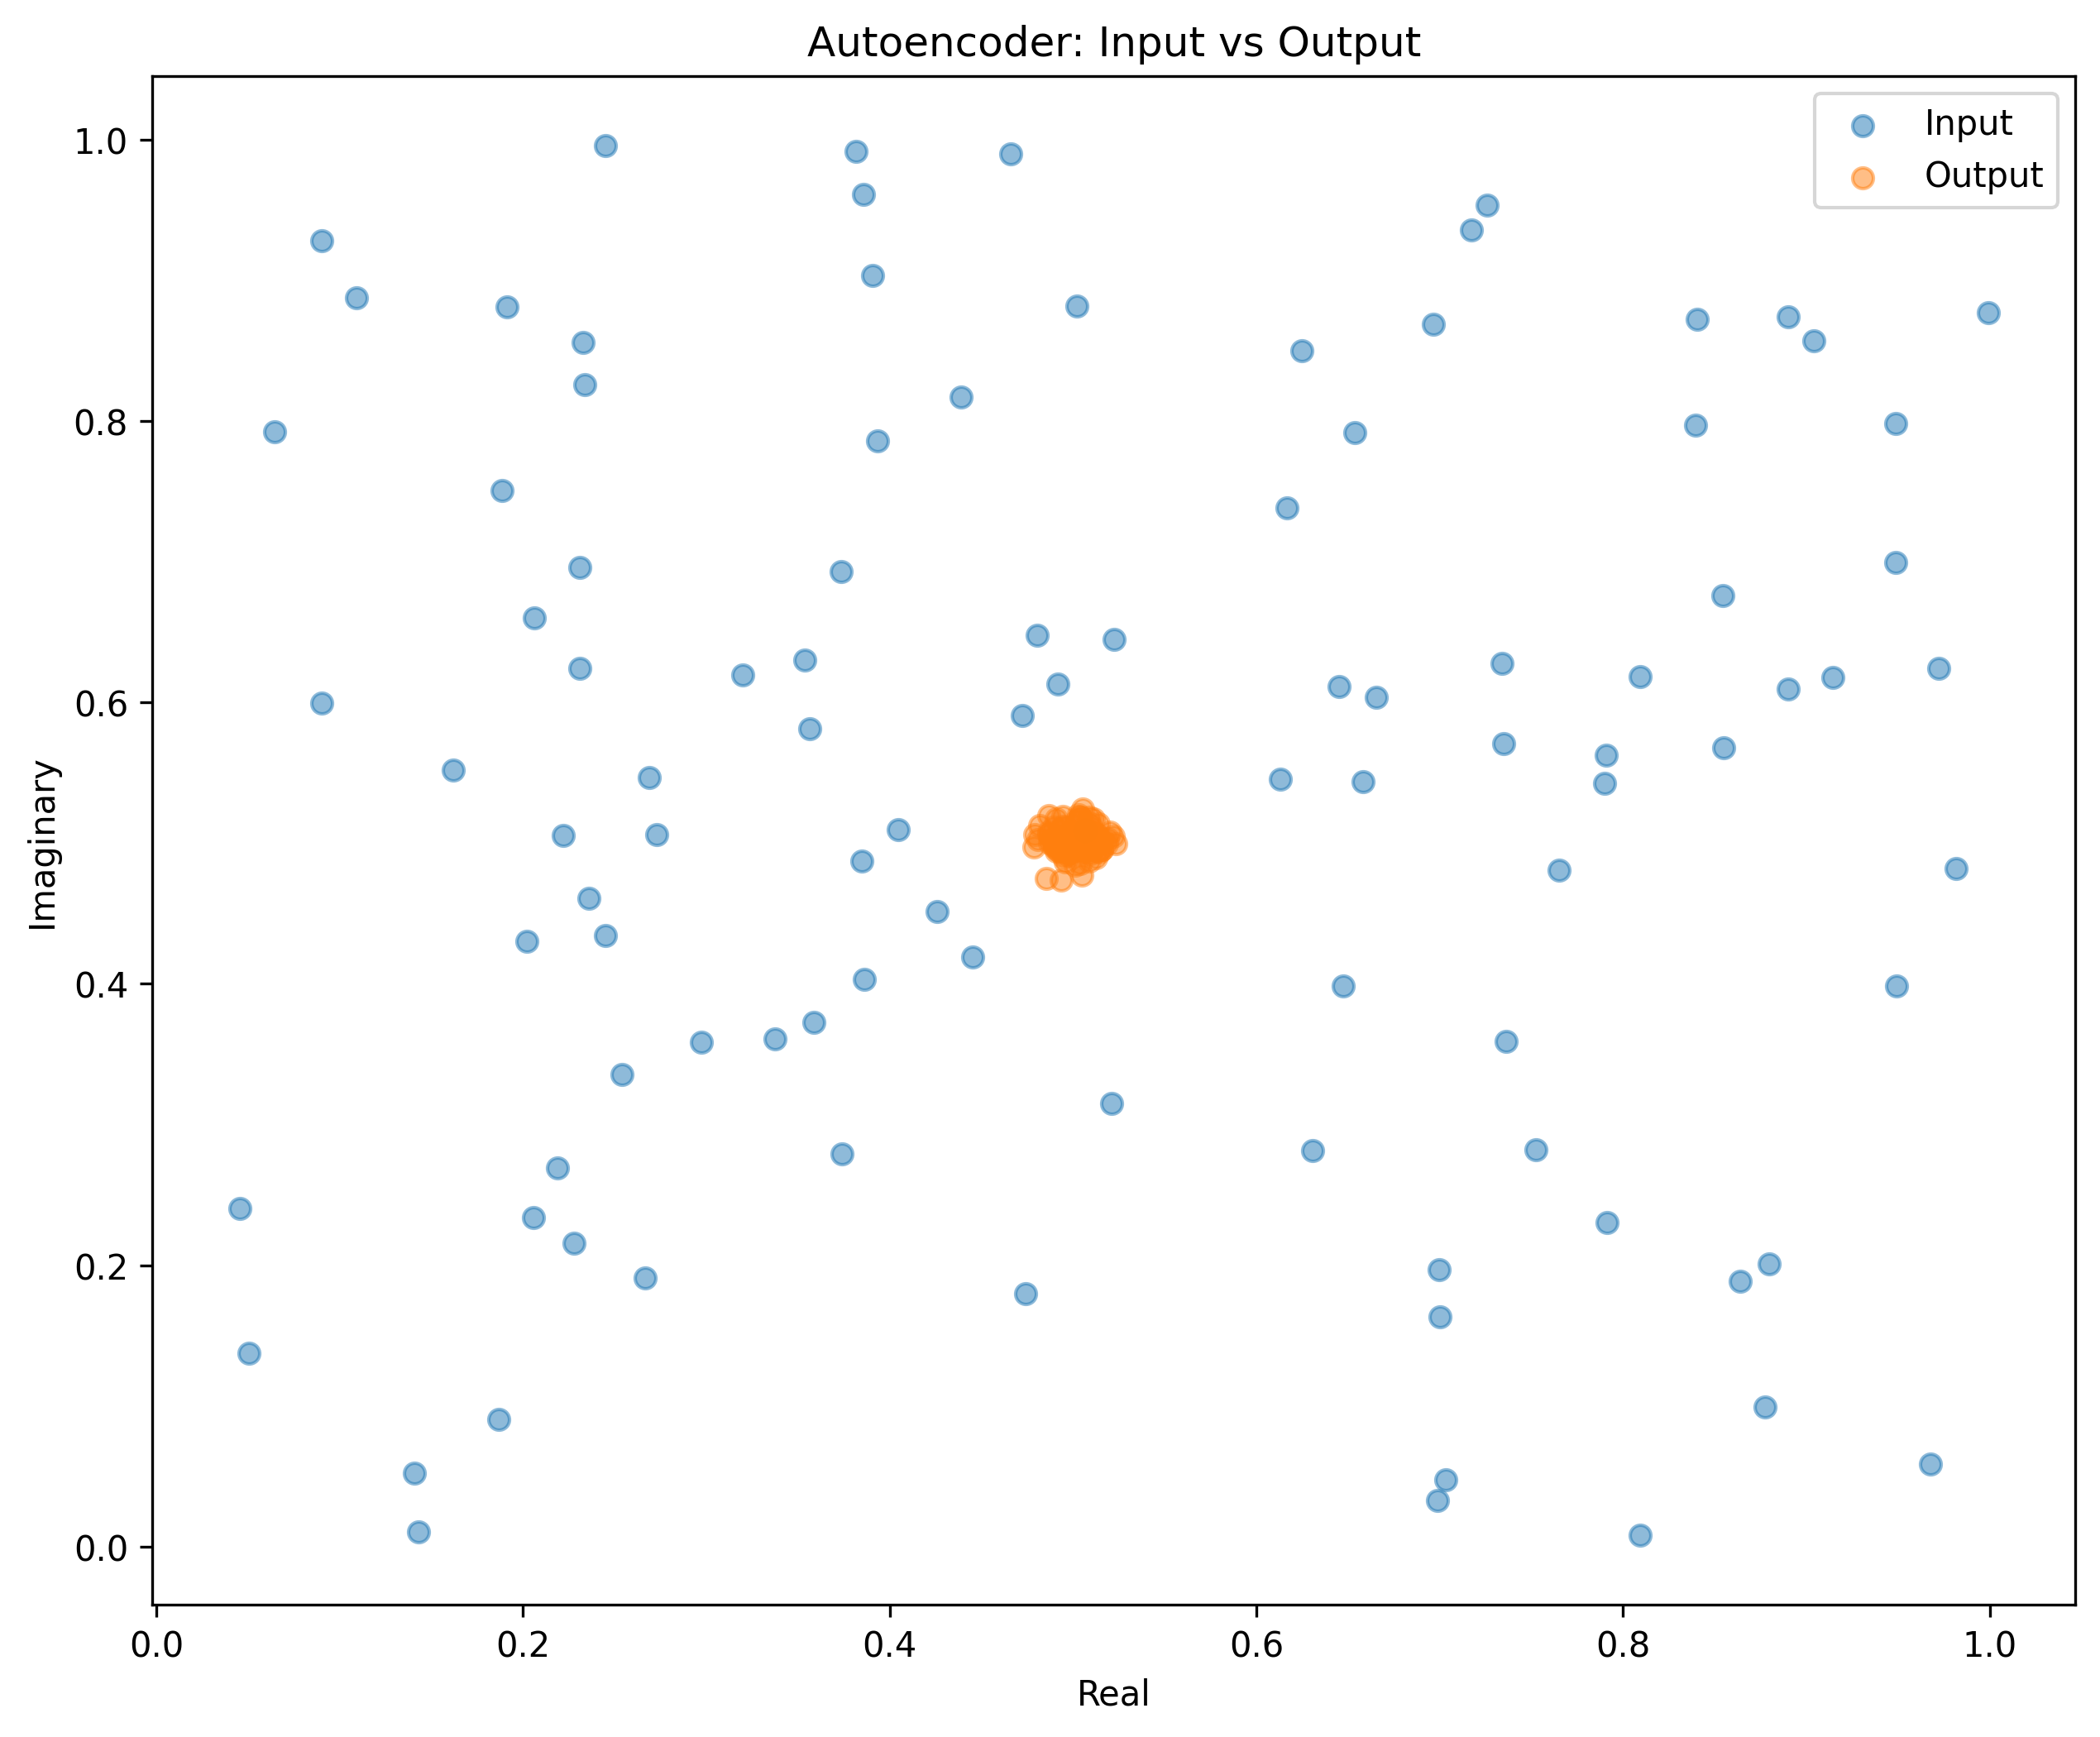
\includegraphics[width=1\linewidth]{autoencoder_comparison.png}
    \caption{Comparison of Autoencoder Performance}
    \label{fig:autoencoder_comparison}
\end{figure}

\paragraph{Direct Transmission Comparison}
Figure \ref{fig:direct_transmission_comparison} shows the comparison between direct transmission and autoencoder-based transmission.

\begin{figure}
    \centering
    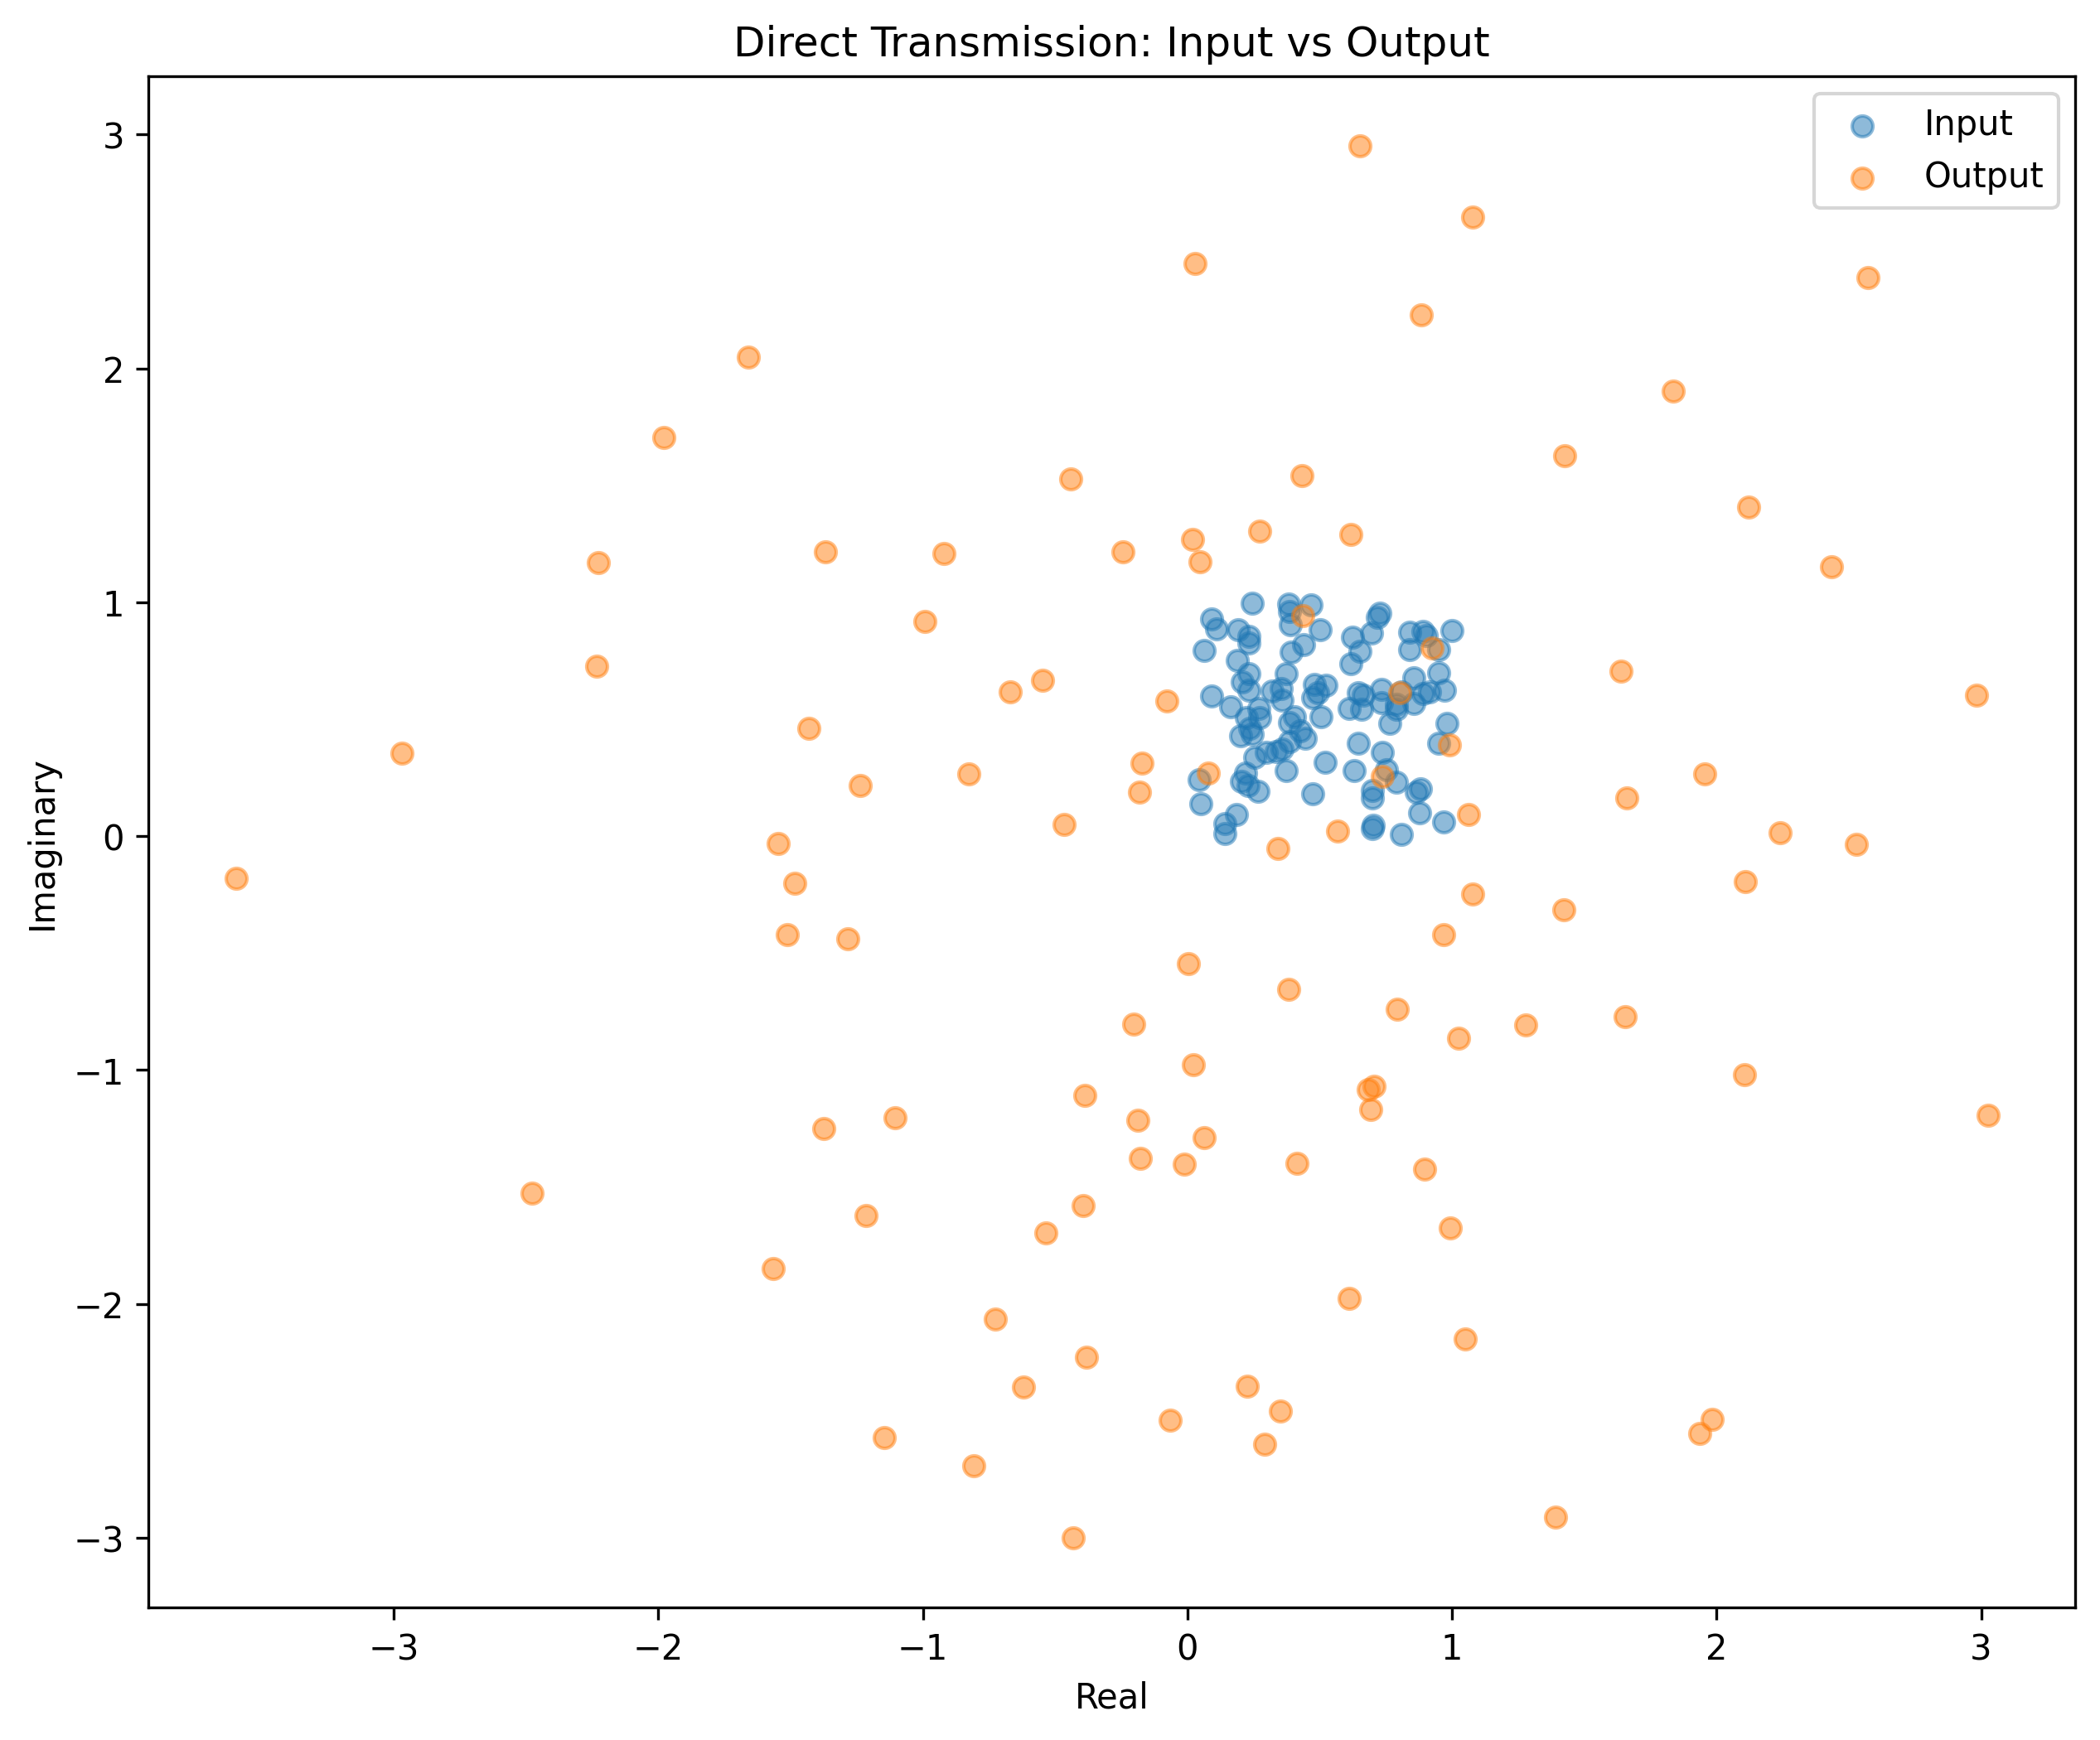
\includegraphics[width=1\linewidth]{direct_transmission_comparison.png}
    \caption{Comparison of Direct Transmission and Autoencoder-Based Transmission}
    \label{fig:direct_transmission_comparison}
\end{figure}

\paragraph{Optical Channel Simulation}
Figure \ref{fig:optical_channel_simulation} illustrates the simulation results of the optical channel.

\begin{figure}
    \centering
    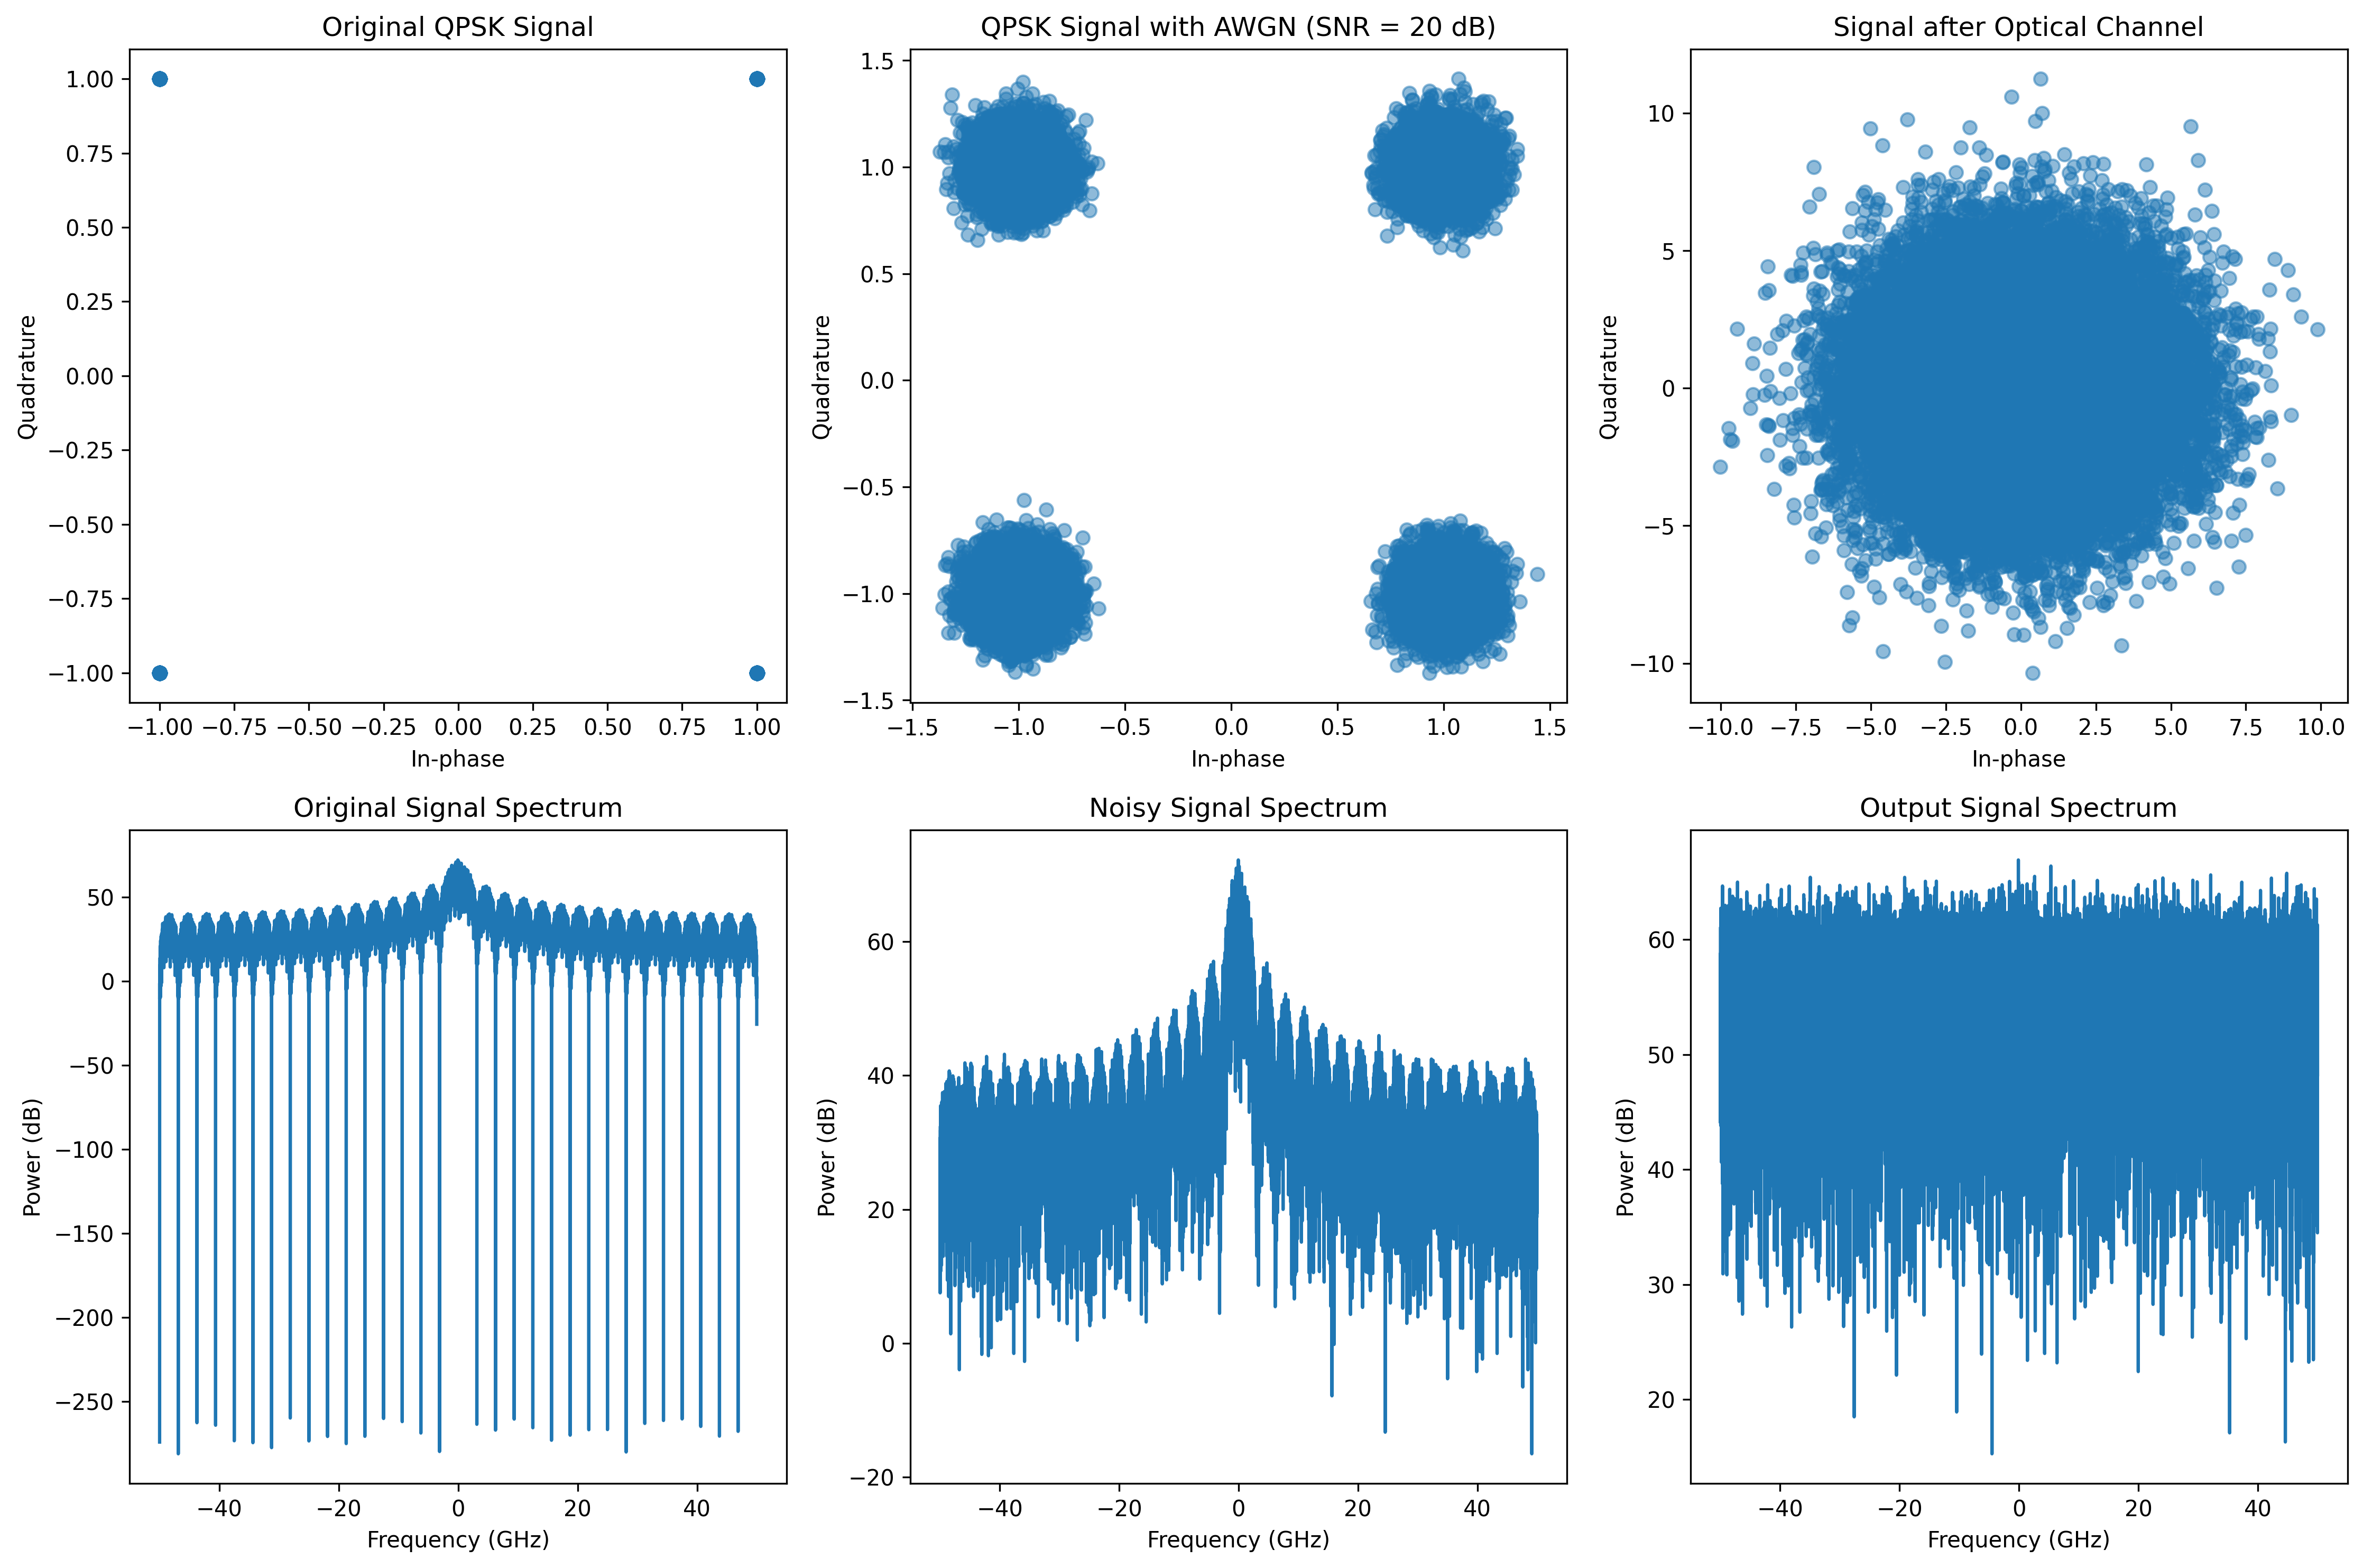
\includegraphics[width=1\linewidth]{optical_channel_simulation.png}
    \caption{Optical Channel Simulation Results}
    \label{fig:optical_channel_simulation}
\end{figure}

\paragraph{Performance Comparison}
Figure \ref{fig:performance_comparison} compares the performance of different models in terms of reconstruction error.

\begin{figure}
    \centering
    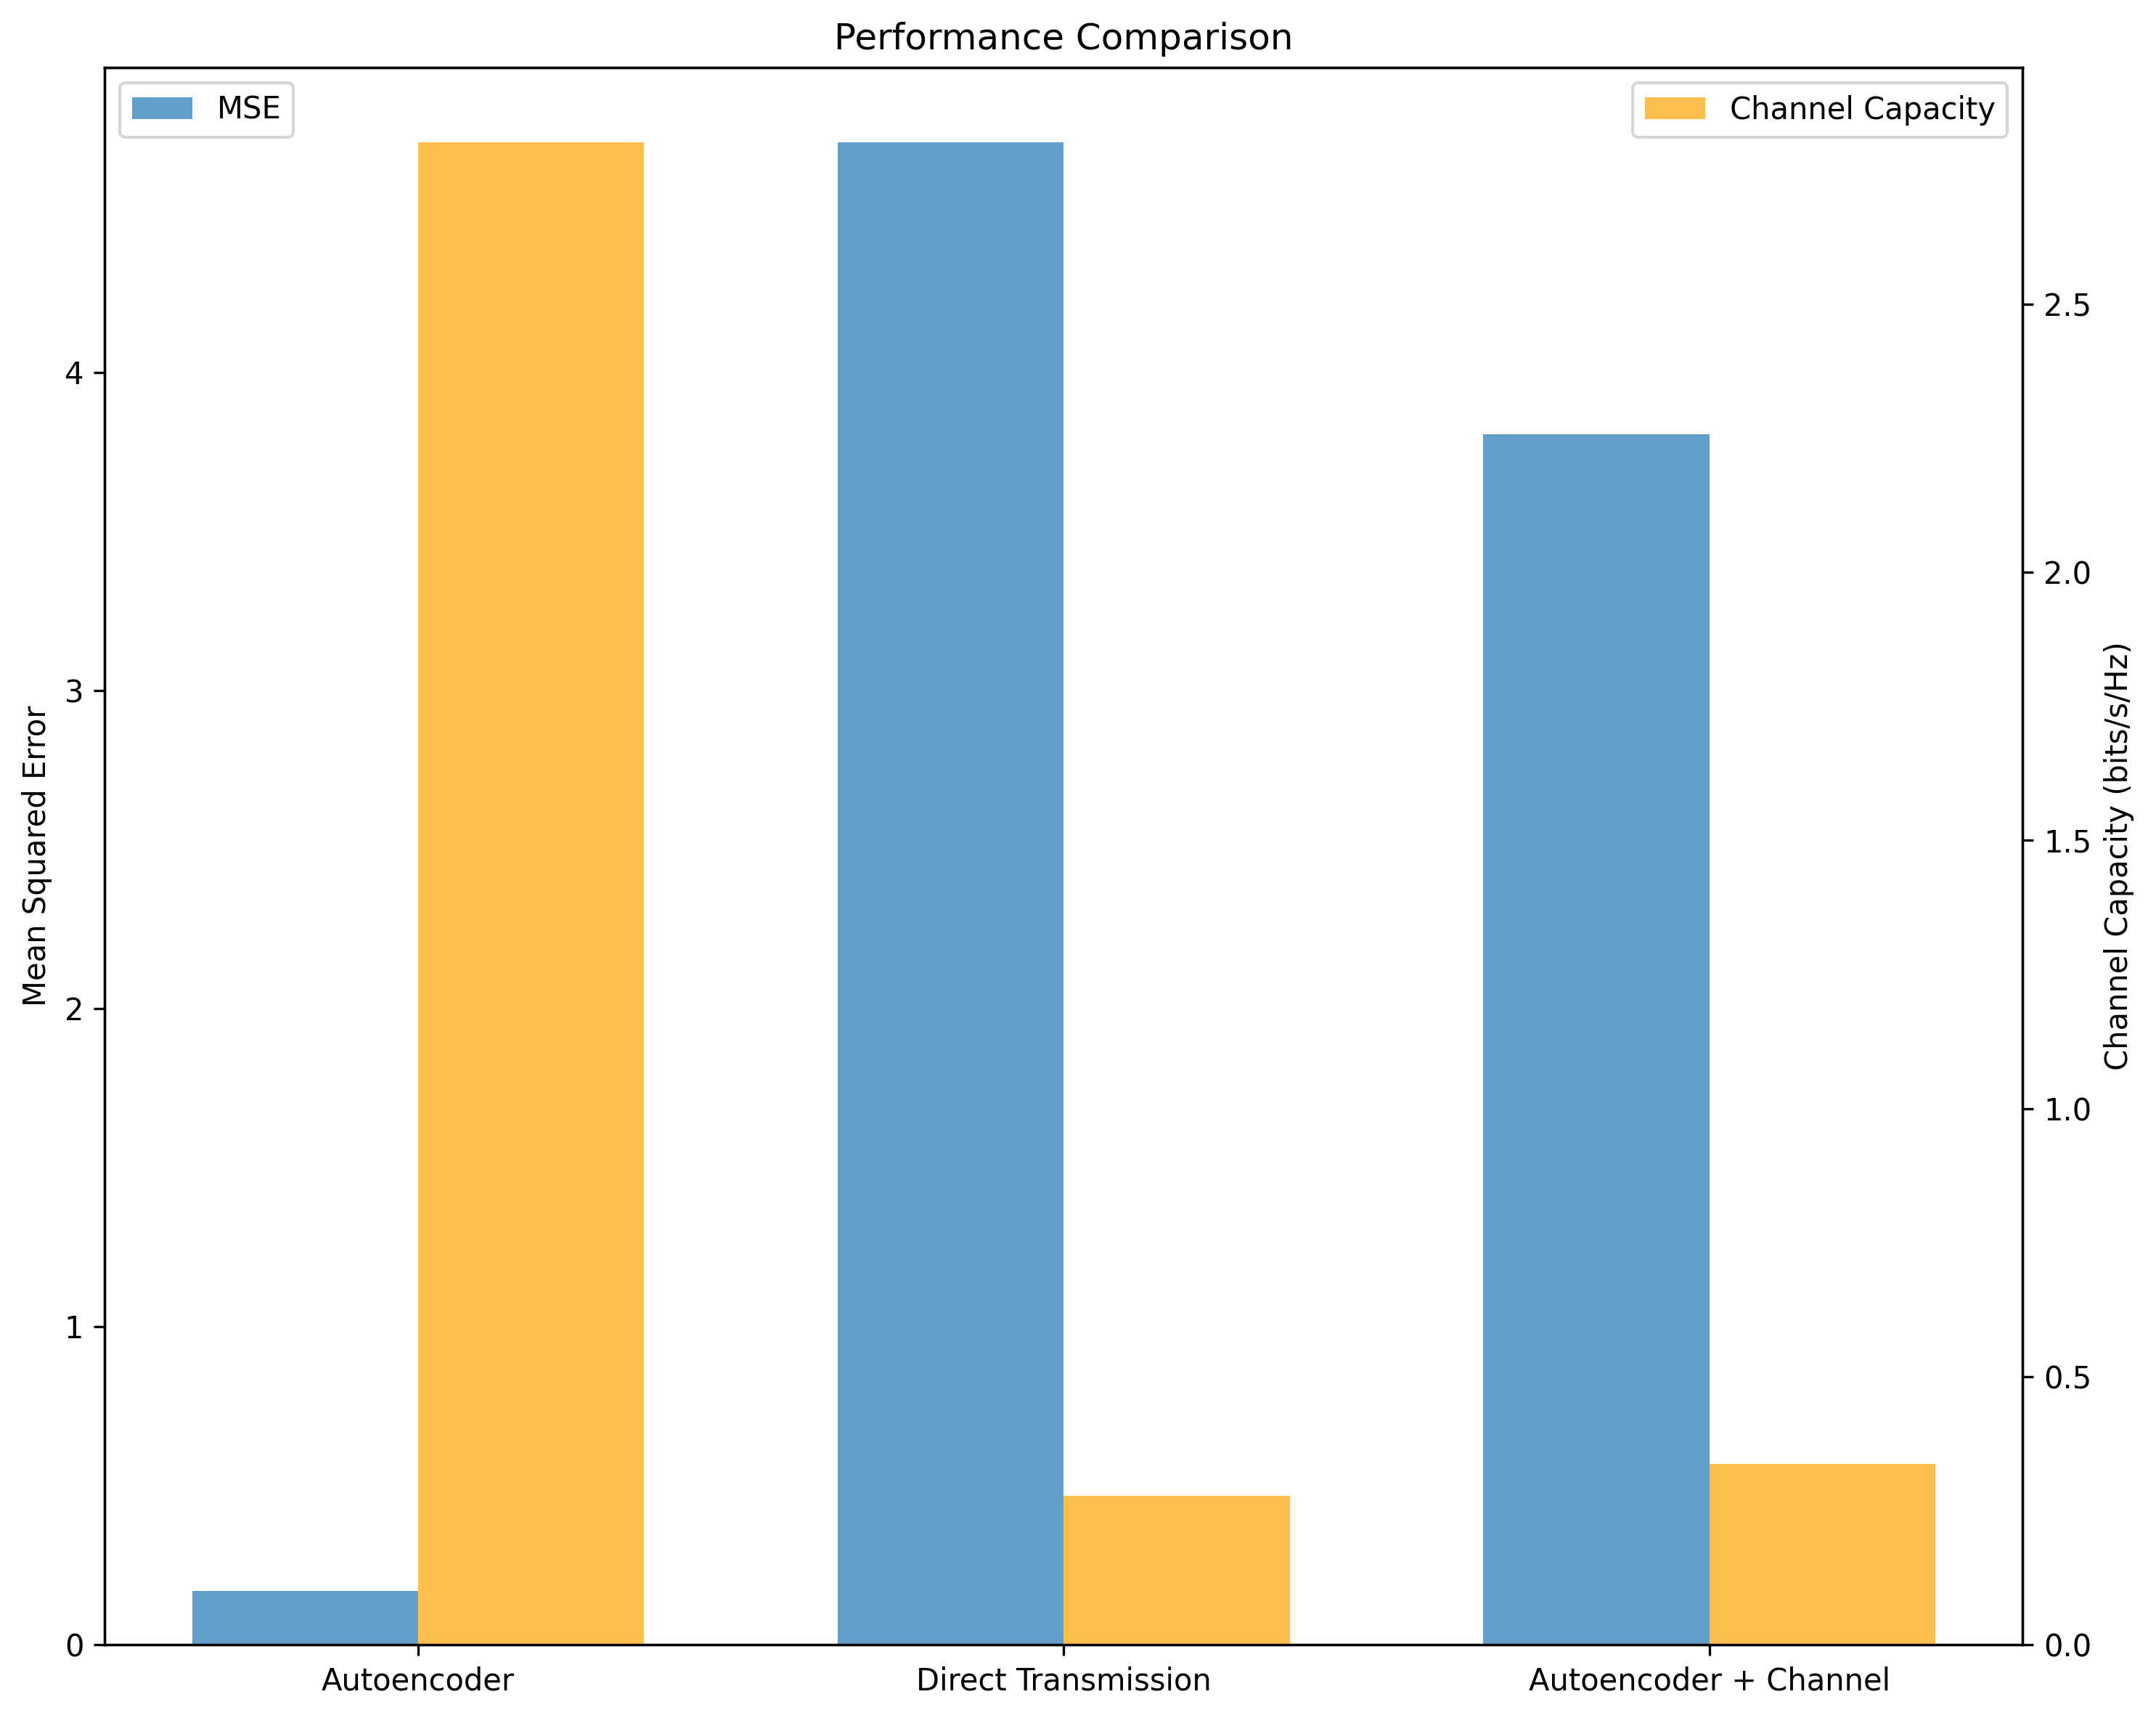
\includegraphics[width=1\linewidth]{performance_comparison.png}
    \caption{Performance Comparison of Different Models}
    \label{fig:performance_comparison}
\end{figure}

\subsubsection{Conclusion}
This report has provided a detailed explanation of the implementation of an autoencoder, including the architecture definition, model training, and performance evaluation. The visual representations of the magnitude distribution and reconstruction error further illustrate the effectiveness of the autoencoder.



















\subsection*{Analysis}

Figure \ref{1} illustrates a comparison of the training and evaluation accuracy for both encoded and raw data across 140 epochs. The plot illustrates the performance of a machine learning model on both the training and evaluation datasets, displaying accuracy scores ranging from 0.1 to 0.9. The figure illustrates the evolution of the training and testing accuracy for a model trained on data that was either left unprocessed or encoded using a proposed MLP algorithm. The raw data was directly transmitted through an optical channel, while the encoded data underwent processing by the MLP network, neural network training, and then transmission through an optical channel. The close proximity of the performance of the training and evaluation sets indicates that the training was effective and there is a low risk of overfitting. After approximately 80 epochs of training, the encoded method achieved an impressive accuracy of 80\(\%\) and showed a tendency to converge.

Figure \ref{2} illustrates the quantity of valid images that can be reconstructed at the receiver, given a fixed data throughput. It is evident that the encoded method significantly enhances data transmission efficiency. Figure \ref{3} presents the ratio derived from Figure \ref{2}, representing the number of bits recoverable at the receiver per bit transmitted. After sufficient training, the encoded method can achieve a transmission efficiency nearly six times that of the baseline. Notably, this ratio can be further increased by adjusting the data compression rate. In this example, images were compressed from their original 28x28 pixels to 125. However, higher compression rates demand more training and introduce a greater risk of overfitting. 

The optimisation algorithm I proposed for applying MLP to optical channels can significantly improve communication efficiency in general cases, i.e., without specific task optimisation or additional noise processing. Different compression rates are suitable for different specific tasks, and further optimisations can be made for particular scenarios.
\begin{figure}
    \centering
    \includegraphics[width=1\linewidth]{2.png}
    \caption{Reconstructed Images Comparison}
    \label{2}
\end{figure}

\begin{figure}
    \centering
    \includegraphics[width=1\linewidth]{3.png}
    \caption{Efficiency Ratio}
    \label{3}
\end{figure}



\section{Future work}
During the next six months of the secondment under the EU H2020 MSCA-RISE grant, I will continue the following research.

\subsection{Channel Modeling Refinement}
Next, I will refine the content related to fibre optic communication channel simulation and package it into a more widely applicable project, with a specific focus on tailoring the model for semantic communication in optical systems. This will involve consolidating the various channel effects (such as chromatic dispersion, polarisation mode dispersion, Kerr effect, and four-wave mixing) into a comprehensive, modular framework. The goal is to create a versatile tool that can be easily integrated into other optical communication research projects, particularly those involving semantic communication.

This refined model will not only simulate traditional optical channel effects but also incorporate features that are crucial for semantic communication, such as:

\begin{itemize}
    \item Adaptive modulation schemes that can adjust based on the semantic importance of the transmitted information
    \item Channel estimation techniques that consider the impact of optical effects on semantic fidelity
    \item Error correction mechanisms tailored to preserve semantic content rather than just bit-level accuracy
    \item Modeling of the interaction between optical channel impairments and semantic information degradation
\end{itemize}

By developing this specialized channel model, I aim to provide researchers in the field of semantic optical communication with a realistic simulation environment that accurately represents the unique challenges and opportunities presented by transmitting semantic information over optical channels. This tool will enable more accurate evaluation of semantic communication protocols and algorithms in the context of optical fibre systems, potentially leading to novel insights and optimizations.

I plan to submit this work to Optics Express, a high-impact journal that covers a wide range of optics and photonics topics. This venue will allow me to reach a broad audience of researchers working at the intersection of optical communications and semantic information processing, fostering further advancements in this emerging field.
\subsection{Integration of Autoencoder with Semantic Optical Communication}
I plan to combine semantic optical communication with autoencoder architectures. Autoencoders are particularly well-suited for this application due to their ability to learn efficient data representations. Their encoder-decoder structure naturally aligns with the concept of semantic communication, where the encoder can learn to extract and transmit only the most relevant semantic information, while the decoder reconstructs the original message from this compressed representation. This approach could significantly enhance the efficiency of semantic communication in optical systems by reducing the amount of data transmitted while preserving the essential meaning. I intend to submit this research to IEEE Transactions on Communications.

\subsection{Applying Diffusion Models to Semantic Optical Communication}
Another promising avenue for research is the integration of diffusion models with semantic optical communication. Diffusion models, known for their ability to generate high-quality samples by gradually denoising data, could be adapted to the semantic communication paradigm. In this context, the diffusion process could be used to gradually refine and reconstruct semantic information at the receiver, potentially improving robustness against channel impairments and noise. This approach could be particularly beneficial in scenarios where the transmitted semantic information is degraded during transmission through the optical channel. I aim to submit this work to IEEE Transactions on Signal Processing, a leading journal in the field of signal processing theory and methods.

\subsection{Development of Semantic Communication Networks}
Current semantic communication models are largely limited to one-to-one scenarios, which do not reflect real-world communication networks. To address this limitation, I propose to investigate the construction of semantic communication networks. This research will explore how semantic information can be efficiently routed and processed in multi-node networks, considering aspects such as:

\begin{itemize}
    \item Semantic routing protocols that can direct information based on its meaning rather than just its destination address
    \item Network architectures that can aggregate and distill semantic information from multiple sources
    \item Scalability of semantic processing in large-scale networks
    \item Handling of semantic conflicts or ambiguities in network nodes
    \item Integration of semantic security measures to protect the meaning of transmitted information
\end{itemize}

This work will aim to bridge the gap between theoretical semantic communication models and practical, large-scale communication systems, paving the way for more intelligent and efficient network infrastructures. I plan to submit this research to IEEE Network, a journal that focuses on novel and emerging topics in networking.






\section*{Acknowledgment}
This code is based on the Semantic-Communication-Systems repository on GitHub, which was created by mxtao at SJTU.
\appendices

\ifCLASSOPTIONcaptionsoff
  \newpage
\fi
\bibliography{references}
\bibliographystyle{ieeetr}
\end{document}


